\documentclass{article}
\newsavebox{\oldepsilon}
\savebox{\oldepsilon}{\ensuremath{\epsilon}}
\usepackage[minionint,mathlf,textlf]{MinionPro} % To gussy up a bit
\renewcommand*{\epsilon}{\usebox{\oldepsilon}}
\usepackage[margin=1in]{geometry}
\usepackage{graphicx} % For .eps inclusion
%\usepackage{indentfirst} % Controls indentation
\usepackage[compact]{titlesec} % For regulating spacing before section titles
\usepackage{adjustbox} % For vertically-aligned side-by-side minipages
\usepackage{array, amsmath,  mhchem}
\usepackage[hidelinks]{hyperref}
\usepackage{courier, subcaption}
\usepackage{multirow, enumerate}
\usepackage[autolinebreaks,framed,numbered]{mcode}
\usepackage{float}
\restylefloat{table}

\pagenumbering{gobble} 
\setlength\parindent{0 cm}
\renewcommand{\arraystretch}{1.2}
\begin{document}
\large

MCB 135 Problem Set 8 \hfill Due Friday, April 10, 2015 at 2:30 PM

\section*{Problem 1: Fluorescence Recovery After Photobleaching (40 points)}

A protein's localization can be used to regulate its activity. Fluorescence Recovery After Photobleaching (FRAP) is one method to investigate whether a protein is diffusing freely or physically confined. The coding sequence of a fluorescent protein is appended to the open reading frame of the protein of interest. A small region of a cell expressing this construct is then photobleached so that all proteins in that region permanently lose fluorescence. Diffusion of nearby fluorescent proteins into the region gradually restores fluorescence. This problem will guide you through a calculation of the expected spatiotemporal profile of fluorescence recovery for diffusion in one dimension, which can be compared to experimental data to estimate the protein's diffusion coefficient.
\begin{enumerate}[a)]
\item Consider the initial concentration profile:
\[ c(x,t=0) = \left\{
     \begin{array}{lr}
       0 & : x < 0\\
       a & : x \geq 0
     \end{array}
   \right. \]
Using the fact that the ``impulse response function" for 1-D diffusion from a point source is $h(x,t)=e^{-x^2/4Dt}/\sqrt{4\pi D t}$, show via convolution that:
\[ c(x,t) = \frac{a}{2} \left[ 1 + \textrm{erf} \left( \frac{x}{\sqrt{4Dt}} \right)\right], \hspace{3 cm} \textrm{ where }\textrm{erf} \left( z \right) \triangleq \frac{2}{\sqrt{\pi}} \int_0^z e^{-u^2} \, du \]
{\color{red}
The profile for $t>0$ is given by the convolution of the initial concentration profile with the impulse response function/Green's function:
\begin{eqnarray*}
c(x,t) & = & \int_{-\infty}^{\infty} c(s,0) h(x - s,t) \, ds\\
& = & a \int_{0}^{\infty} h(x-s,t) \, ds = \frac{a}{\sqrt{4\pi D t}} \int_0^{\infty} e^{-\frac{(x-s)^2}{4Dt}} \, ds  \\
\end{eqnarray*}
To simplify, we define:
\[ u = \frac{x-s}{\sqrt{4Dt}} \hspace{3 cm} du = - \frac{ds}{\sqrt{4Dt}} \]
As $s \to 0$, $u \to x/\sqrt{4Dt}$; as $s \to \infty$, $u \to -\infty$. With this substitution, we have:
\begin{eqnarray*}
c(x,t) & = & \frac{-a}{\sqrt{\pi}} \int_{x/\sqrt{4Dt}}^{-\infty} e^{-u^2} \, du  = \frac{a}{\sqrt{\pi}} \int_{-\infty}^{x/\sqrt{4Dt}} e^{-u^2} \, du \\
& = & \frac{a}{\sqrt{\pi}} \left[\int_{-\infty}^{0} e^{-u^2} \, du +  \int_{0}^{x/\sqrt{4Dt}} e^{-u^2} \, du \right]\\
& = & \frac{a}{\sqrt{\pi}} \left[\frac{\sqrt{\pi}}{2} +  \frac{\sqrt{\pi}}{2} \textrm{ erf} \left( \frac{x}{\sqrt{4Dt}} \right) \right]\\
& = & \frac{a}{2} \left[1 +  \textrm{ erf} \left( \frac{x}{\sqrt{4Dt}} \right) \right]\\
\end{eqnarray*}
}
\item A region along the axis of a rod-shaped cell is photobleached so that the initial concentration profile is:
\[ c(x,t=0) = \left\{
     \begin{array}{lr}
       0 & : -L < x < L\\
       a & : \textrm{otherwise}
     \end{array}
   \right. \]
Find an expression for $c(x,t)$ in terms of the error function erf(). (Hint:  this can be done without taking any more integrals.)\\

{\color{red}
Notice that we can solve the following related initial value problems by shifting and making a symmetry argument:
\begin{eqnarray*}
c_1(x,t=0) = \left\{
     \begin{array}{lr}
       0 & : x < L\\
       a & : \textrm{otherwise}
     \end{array}
   \right. & \implies & c_1(x,t) = \frac{a}{2} \left[ 1 + \textrm{erf} \left( \frac{x- L}{\sqrt{4Dt}} \right) \right]\\
   c_2(x,t=0) = \left\{
     \begin{array}{lr}
       0 & : x > -L\\
       a & : \textrm{otherwise}
     \end{array}
   \right. & \implies & c_2(x,t) = \frac{a}{2} \left[ 1 - \textrm{erf} \left( \frac{x+L}{\sqrt{4Dt}} \right) \right]\\
   \end{eqnarray*}
The solution to our initial value problem is just the sum of these two solutions:
\[ c(x,t) = c_1(x,t) + c_2(x,t) = \frac{a}{2} \left[ 2 + \textrm{erf} \left( \frac{x-L}{\sqrt{4Dt}} \right)  - \textrm{erf} \left( \frac{x+L}{\sqrt{4Dt}} \right) \right] \]
}

\item Plot $c(x,t)$ from part (b) for $x\in[-20,20]$ at $t=0.01, 1,$ and $100$. Use the parameter values $D=1$, $a=1$, and $L=5$.
\begin{center}
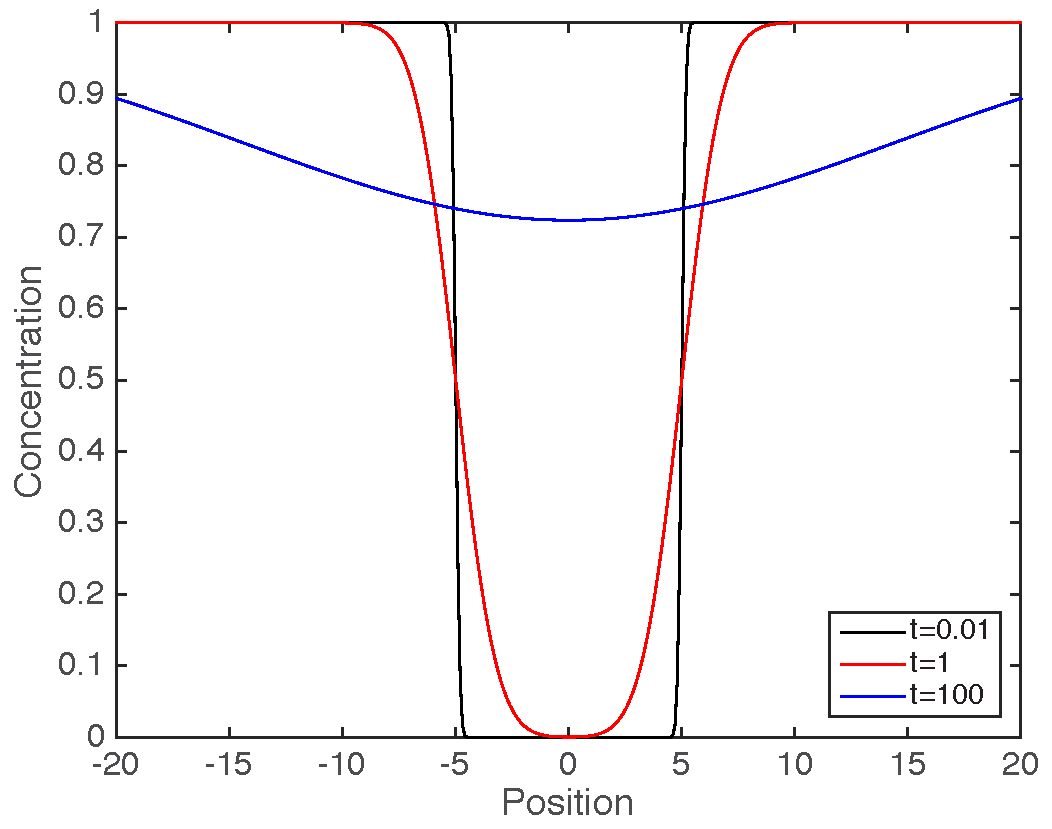
\includegraphics[width=0.5\textwidth]{problem1c.pdf}
\end{center}

\begin{lstlisting}
function [] = problem1c()
    D = 1;
    a = 1;
    L = 5;
    x = -20:0.1:20;
    
    t = 0.01;
    y = (a/2) * (2 + erf((x-L)/(4*D*t)^0.5) - erf((x+L)/(4*D*t)^0.5));
    plot(x,y,'-k'); hold on;
    
    t = 1;
    y = (a/2) * (2 + erf((x-L)/(4*D*t)^0.5) - erf((x+L)/(4*D*t)^0.5));
    plot(x,y,'-r'); 
    
    t = 100;
    y = (a/2) * (2 + erf((x-L)/(4*D*t)^0.5) - erf((x+L)/(4*D*t)^0.5));
    plot(x,y,'-b');
    
    legend('t=0.01','t=1','t=100','Location','SouthEast')
    set(gca,'FontSize',16)
    xlabel('Position')
    ylabel('Concentration')
    
end
\end{lstlisting}

\item Outline how you would estimate $D$ if given a single fluorescence profile collected $\tau$ seconds after photobleaching. You may assume that photobleaching is perfectly efficient, and that $L$ and $x$ are known.\\

{\color{red}
Multiple answers are acceptable. One approach would be:
\begin{enumerate}[i)]
\item Estimate the parameter $a$ as the fluorescence at a distance far from the site of photobleaching
\item Calculate the expected fluorescence profile at each measured point for a range of values of $D$ using the formula
\item Compute the sum of squared error $\sum (\textrm{ Expected } - \textrm{ Observed })^2$ for each of these values of $D$, and
\item Choose the value of $D$ with the smallest sum of squared error (or repeat steps 2-4 with an improved range of values for $D$)
\end{enumerate}
}

\end{enumerate}

\section*{Problem 2: Epidemic (60 points)}
A disease spreads through a population of $N$ persons: $x$ of them are infected, and the remainder, $s=N-x$, are susceptible. When the infection subsides, a person becomes susceptible again (no immunity is conferred). Infection and recovery are modeled by two events:
\[ \ce{X + S ->[k_1] X + X} \hspace{3 cm} \ce{X ->[k_2] S}  \]

\begin{enumerate}[a)]
\item What is the analog of the system size $\Omega$ in this model?\\
{\color{red}
$N$, the population size, is the analog of $\Omega$ for this system.
}

\item What is the stoichiometry matrix for these events?\\
{\color{red}
Maintaining the order of events given above,
\[ S = \begin{pmatrix} 1 & -1 \end{pmatrix} \]
}

\item What are the two event propensities $\Omega r_i(x, \Omega)$?
{\color{red}
\begin{eqnarray*} P_1 & = & N r_1(x,N) = N k_1 \left( \frac{x}{N} \right)\left( \frac{N - x}{N} \right) = \frac{k_1 x(N-x)}{N}\\
P_2 & = & N r_2(x,N) = N k_2 \left( \frac{x}{N} \right) = k_2 x
\end{eqnarray*}
}


\item Using your answers to (a)-(c), find expressions for the first and second jump moments, $\mu(x,t)$ and $\sigma^2(x,t)$.
{\color{red}
\begin{eqnarray*} \mu(x,t) & = & \sum_{k=1}^2 s_k P_k = \frac{k_1 x(N-x)}{N} - k_2 x\\
\sigma^2(x,t) & = & \sum_{k=1}^2 s_k s_k^T P_k = \frac{k_1 x(N-x)}{N} + k_2 x
\end{eqnarray*}
}

\item Write down an expression for $dx$ in Langevin notation.
{\color{red}
\[ dx = \mu(x,t) \, dt + \sigma(x,t) \, dW_t = \left[ \frac{k_1 x(N-x)}{N} - k_2 x \right] \, dt + dW_t \sqrt{\frac{k_1 x(N-x)}{N} + k_2 x} \]
}

\item Simulate the system using the Euler-Maruyama method with parameters $N=1000$, $k_1 = 0.2$, and $k_2 = 0.1$ and with step size $\Delta t = 0.1$ and $t \in [0,1000]$. Include a plot with three sample trajectories with initial values $x(0)=100,500,$ and $900$.
{\color{red}
We first rewrite to clarify that the step size for the simulation will be found using:
\[ \Delta x =  \left[ \frac{k_1 x(N-x)}{N} - k_2 x \right] \, \Delta t + \eta \, \sqrt{\Delta t} \sqrt{\frac{k_1 x(N-x)}{N} + k_2 x} \]
where $\eta \sim \mathcal{N}(0,1)$.
\begin{center}
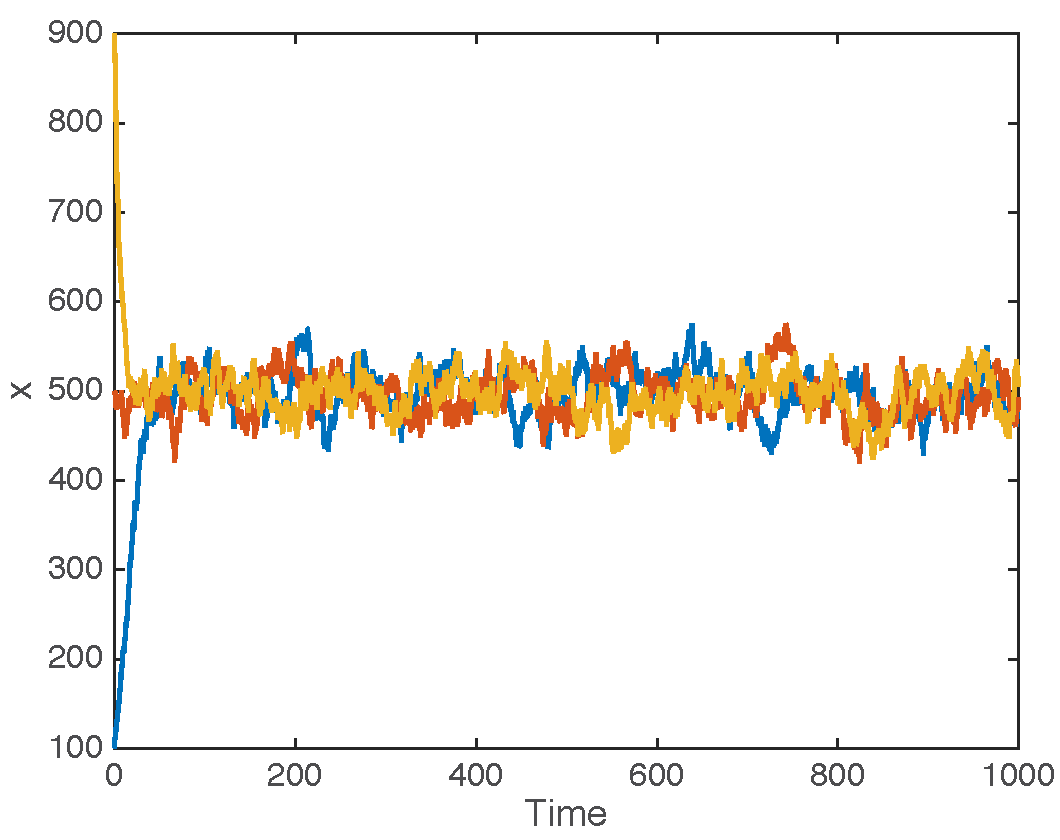
\includegraphics[width=0.5\textwidth]{problem2f.pdf}
\end{center}
}
\begin{lstlisting}
function [] = problem2f()
    k1 = 0.2;
    k2 = 0.1;
    N = 1000;
    
    delta_t = 0.1;
    t = 0:delta_t:1000;
    x0= [100 500 900];
    for i=1:3
        x = zeros(1,length(t)); x(1) = x0(i);
        for j=2:length(t)
            x(j) = x(j-1) + ((k1/N)*x(j-1)*(N - x(j-1)) - k2*x(j-1))*delta_t + ...
                ((k1/N)*x(j-1)*(N - x(j-1)) + k2*x(j-1))^0.5 *(delta_t^0.5)*normrnd(0,1);
            if x(j) > N
                x(j) = N;
            elseif x(j) < 0
                x(j) = 0;
            end
        end
        plot(t,x,'LineWidth',2); hold on;
    end
 
    xlabel('Time')
    ylabel('x')
    set(gca,'FontSize',16)
    
end
\end{lstlisting}

\item Use Wright's formula to find an expression proportional to the stationary probability distribution of states, $P(x)$. Do not calculate the normalization constant. Hint: to save headaches later, don't omit the absolute value notation when taking integrals of the form  $\int \frac{dx}{x} = \ln |x|+C$.

{\color{red}
According to Wright's formula,
\begin{eqnarray*}
P(x,t) & \propto &  \frac{1}{\sigma^2} \exp \left( \int \frac{\mu}{\sigma^2} \, dx  \right) = \frac{1}{ \frac{k_1 x(N-x)}{N} + k_2 x} \exp \left( \int \frac{ \frac{k_1 x(N-x)}{N} - k_2 x}{ \frac{k_1 x(N-x)}{N} + k_2 x} \, dx  \right)\\
& = & \frac{N}{ k_1 x(N-x) + k_2 N x}    \exp \left( \int \frac{ k_1 (N-x) - k_2 N}{ k_1 (N-x) + k_2 N} \, dx  \right)\\
& = & \frac{N}{ k_1 x(N-x) + k_2 N x}    \exp \left( \int 1 - \frac{ 2 k_2 N}{ k_1 (N-x) + k_2 N} \, dx  \right)\\
& = & \frac{N}{ k_1 x(N-x) + k_2 N x}    \exp \left( x + 2 k_2 N \int  \frac{ 1}{ k_1 x - (k_1 + k_2) N} \, dx  \right)\\
& = & \frac{Ne^x}{ k_1 x(N-x) + k_2 N x}    \exp \left( \frac{ 2 k_2 N}{k_1} \ln \left| k_1 x - (k_1 + k_2) N \right|   \right)\\
& = & \frac{Ne^x}{ k_1 x(N-x) + k_2 N x} \left| k_1 x - (k_1 + k_2) N \right|^{ \frac{ 2 k_2 N}{k_1} }\\
 \end{eqnarray*}
Note that the quantity inside of the absolute value sign is guaranteed to be negative.
}

\item In the real world, what would happen if $x$ chances to reach zero? How does this reflect what will happen if you attempt to normalize your expression for $P(x)$ over $x \in [0, N] \cap \mathbb{Z}$?\\
{\color{red}
If $x$ reaches zero, no people will be infected and the disease will be eliminated (unless it has a natural reservoir). Notice that the expression of $P(x,t)$ goes to infinity as $x \to 0$: this indicates that the normalized probability distribution is $P(x,t)=\delta(x)$, i.e., the stationary probability distribution is $x=0$.
}
\end{enumerate}
As you saw in part f, this system has a different, ``pseudo-stable" behavior that is apparent on intermediate timescales. We can investigate it by normalizing $P(x)$ over all $x \neq 0$.
\begin{enumerate}[a)]
\setcounter{enumi}{8}
\item Numerically calculate $P^*(x)$, the ``pseudo-stationary probability distribution," by normalizing $P(x)$ with the parameter values given above for $x \in [1, N] \cap \mathbb{Z}$.  Hint: to minimize rounding errors, calculate $\ln P(x)$ for each value of $x$, subtract the minimum value in this array from all values in the array, then exponentiate and normalize.\\
\begin{lstlisting}
    lnp = zeros(1,N);
    for x=1:N
        lnp(x) = -1 * log(1/((k1/N)*x*(N - x) + k2*x)) + x + ...
            (2*k2*N/k1) * log(abs(k1*x - (k1+k2)*N));
    end
    lnp = lnp - min(lnp);
    p = exp(lnp);
    p = p ./ sum(p);
\end{lstlisting}
\item Calculate the mean $m$ and standard deviation $s$ of $P^*(x)$.
\begin{lstlisting}
    p_mean = 0;
    p_variance = 0;
    for x=1:N
       p_mean = p_mean + x*p(x);
       p_variance = p_variance + (x^2)*p(x);
    end
    p_variance = p_variance - p_mean^2;
    p_std_dev = p_variance^0.5;
\end{lstlisting}
\item Add lines to your plot from part (f) to mark $x=m-2s$ and $x=m+2s$. Do your simulated trajectories tend to remain within these bounds after reaching the pseudo-stationary distribution?\\
{\color{red} The trajectories tend to remain within two standard deviations of the mean on this timescale. }
\begin{center}
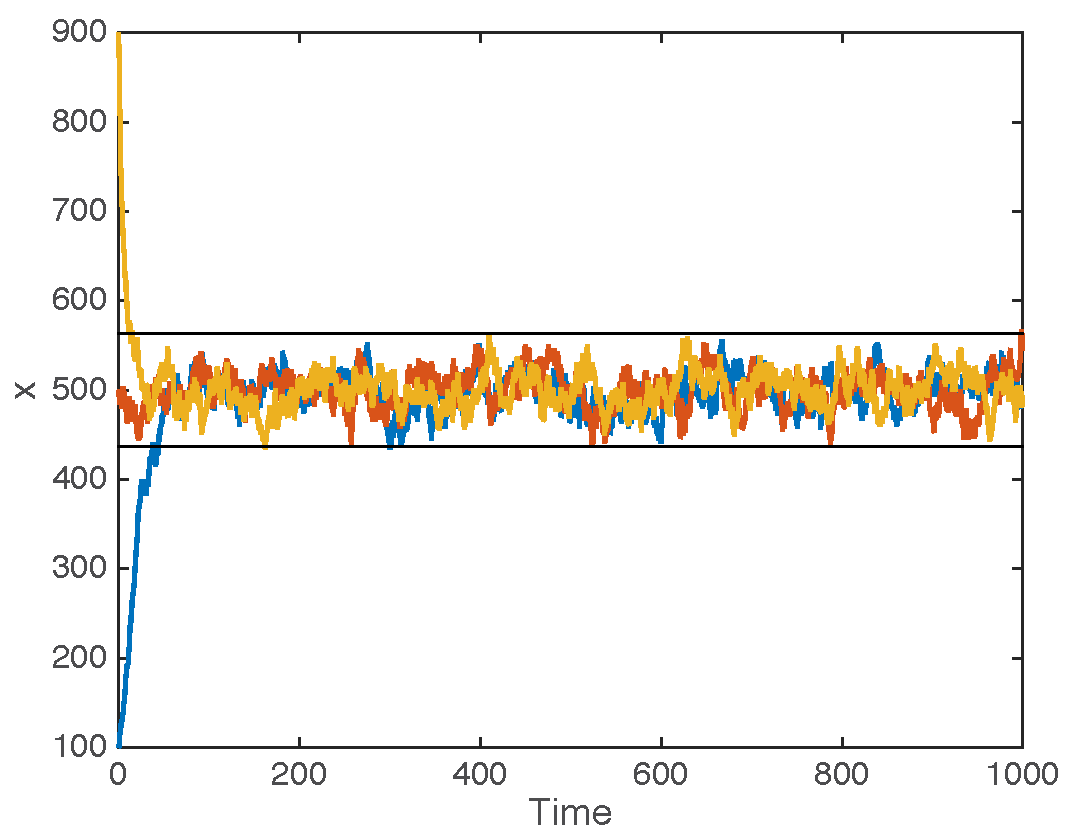
\includegraphics[width=0.5\textwidth]{problem2j.pdf}
\end{center}
\begin{lstlisting}
    plot([0, t(end)],[p_mean - 2 * p_std_dev, p_mean - 2 * p_std_dev],'k')
    plot([0, t(end)],[p_mean + 2 * p_std_dev, p_mean + 2 * p_std_dev],'k')
\end{lstlisting}

\end{enumerate}

\end{document}